\chapter{Metodologia}

Este Capítulo apresenta a estrutura geral do sistema, a configuração inicial do RaspberryPi, a construção dos microsserviços, assim como as etapas de realização do projeto. A
primeira etapa consiste no desenvolvimento do microsserviço de cadastro e controle de usuários. Em seguida, foi desenvolvido o sistema que recebe os dados via MQTT, guardando-os no InfluxDB. Com os dados sendo recebidos e devidamente guardados, foi configurado o HomeAssistant juntamente com o Grafana.

A validação do projeto será feita através de um sistema criado para emular os dados vindos dos sensores, atuadores e teclado. Este sistema é capaz de criar dados que simulam os sinais recebidos pelo sensor YF-S201, pelo teclado numérico e atuador.

\section{Funcionamento do sistema}

Nesta seção estão descritos o funcionamento do sistema, os parâmetros utilizados nele assim como as respostas esperadas.

\subsection{Parâmetros de operação}

Aqui são apresentados e explicados os parâmetros de operação e como eles ditam o funcionamento do sistema. Estes parâmetros são:

\begin{itemize}
	\item Tempo de banho permitido: é o tempo máximo de banho permitido para cada usuário;
	\item Estado do chuveiro: ligado ou desligado;
	\item Estado do usuário: autorizado ou não autorizado;
\end{itemize}

Ao se criar um usuário é necessário informar três dados: nome do usuário, senha e tempo de banho permitido. A senha é utilizada para autorizar o usuário a tomar o banho, para iniciar o banho, o usuário deve digitar sua senha no teclado numérico. O tempo de banho permitido é o tempo máximo em que o chuveiro pode ficar ligado, ao exceder este limite, o atuador irá interromper o fluxo de água.

O estado do chuveiro poderá ser observado no HomeAssistant, que dirá se o usuário está com o chuveiro ligado ou desligado. Cada usuário terá sua própria informação do seu sensor no HomeAssistant.

\subsection{Dados gerados}

O usuário, ao digitar a sua senha correta no teclado numérico, liberará o atuador e o fluxo de água começará a passar pelo sensor de fluxo. Este sensor irá gerar dados que dizem informações a respeito da quantidade de água por segundo que está passando por ele.

Os dados do sensor são gravados no InfluxDB e poderão ser vistos no Grafana em forma de gráfico, sendo possível distinguir os usuários. O sistema, ao perceber uma parada no fluxo, ou se o tempo de banho ultrapassar o limite de banho do usuário, fecha o atuador e contabiliza o tempo total do banho tomado guardando-o no Banco de Dados PostgreSQL.

\subsection{Ligar/desligar atuador}

Para ligar o atuador, o sistema precisa identificar o usuário e autentica-lo. A identificação e autenticação do usuário é realizada via teclado numérico. O usuário é identificado pelo seu id, que é fornecido no momento do seu cadastro. Para realizar a identificação o usuário deve pressionar no teclado a tecla \textit{\*} seguido pelo seu id e em seguida \textit{\#}. Ao realizar a consulta, o sistema retorna o nome do usuário e requisita a senha.

Após digitar a senha, a tecla \textit{\#} deve ser pressionada para o sistema comparar a senha digitada com a cadastrada no banco de dados. Caso as senhas forem iguais, o atuador é ligado, caso forem diferentes, o sistema retorna que o usuário não está autenticado e não liga o atuador. 

A Figura \ref{fig:mockservice} mostra este fluxo de digitação, assim como a identificação do usuário pelo id.

\section{Configuração do RaspberryPi} \label{sec:confrasp}

Para a configuração inicial do RaspberryPi é preciso fazer o download de um sistema operacional compatível com o microcontrolador. Para o sistema deste projeto, utilizamos o Raspbian\footnote{\url{https://www.home-assistant.io/docs/installation/hassbian/installation/}}, que foi instalado no cartão SD a ser inserido no RaspberryPi.


Os sistemas deste projeto foram desenvolvidos diretamente no RaspberryPi, e, para possibilitar este desenvolvimento, é necessário primeiramente configurar o ambiente do RaspberryPi.

O RaspberryPi foi configurado para ser \textit{headless}\footnote{\url{https://www.raspberrypi.org/documentation/configuration/wireless/headless.md}}, o que faz com que ele não necessite de teclado, mouse ou monitor para poder ser acessado. Para conseguir acessar o RaspberryPi nesta configuração é necessária a utilização do SSH, ou \textit{Secure Shell}, que é um protocolo de rede criptográfico para operação de serviços de rede de forma segura\footnote{\url{https://www.ssh.com/ssh/}}. O SSH permite o login remoto no sistema operacional do Raspberry, possibilitando o completo controle do sistema operacional de forma remota.

A configuração de rede do RaspberryPi foi realizada para conter um IP estático (\textit{192.168.2.60}), que facilita o acesso SSH ao sistema.

A Figura \ref{fig:headless} mostra um exemplo do arquivo \textit{wpa\_supplicant.conf}, que faz parte da configuração \textit{headless}, servindo para conectar à rede automaticamente ao iniciar os RaspberryPi. Já na Figura \ref{fig:rpiip}, podemos observar a configuração do ip estático.

\begin{figure}[htbp]
	\centering
	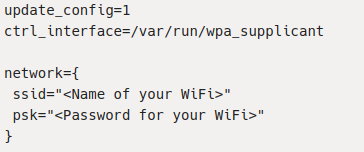
\includegraphics[width=0.6\linewidth]{figuras/headless.png}
	\caption{Exemplo de configuração \textit{headless}}
	\label{fig:headless}
\end{figure}

\begin{figure}[htbp]
	\centering
	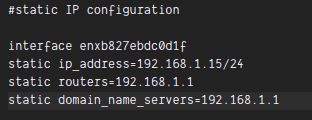
\includegraphics[width=0.6\linewidth]{figuras/rpiip.png}
	\caption{Exemplo de configuração do IP estático}
	\label{fig:rpiip}
\end{figure}

\section{Criação das tabelas no PostgreSQL}

Em bancos de dados relacionais, para salvar os dados é necessário criar um banco de dados com o nome desejado. Dentro do banco, são criadas tabelas que se relacionam entre si, e, dentro das tabelas, existem colunas, referente ao dado que deseja guardar. Nesta seção estão as descrições do banco de dados criado, suas tabelas e colunas.

Para o sistema desenvolvido, foi criado um banco de dados com o nome \textit{users} com três tabelas: \textit{user\_baths}, \textit{user\_settings} e \textit{users}.

A tabela \textit{users} contém 5 colunas, que guardam informações dos usuários cadastrados, que são:
\begin{itemize}
	\item id: gera um id que se auto incrementa e é único para cada usuário;
	\item \textit{name}: referente ao nome do usuário;
	\item \textit{password}: informação da senha do usuário, que é criptografada;
	\item \textit{created\_at}: data e hora da criação do usuário;
	\item \textit{updated\_at}: data e hora da ultima atualização do usuário;
\end{itemize}

A tabela \textit{user\_settings} guarda informações de configuração dos usuários, e também contém 5 colunas:

\begin{itemize}
	\item id: identificador único;
	\item \textit{user\_id}: referente ao id do usuário;
	\item \textit{allowedBathTime}: tempo de banho permitido do usuário;
	\item \textit{created\_at}: data e hora da criação do usuário;
	\item \textit{updated\_at}: data e hora da ultima atualização do usuário;
\end{itemize}

A tabela \textit{userBaths} guarda informações de tempo de todos os banhos tomados, possuindo 5 colunas:

\begin{itemize}
	\item id: identificador único;
	\item \textit{user\_id}: referente ao id do usuário;
	\item \textit{time}: tempo total do banho, em milissegundos;
	\item \textit{created\_at}: data e hora da criação do usuário;
	\item \textit{updated\_at}: data e hora da ultima atualização do usuário;
\end{itemize}

A Figura \ref{fig:erpostgre} mostra o diagrama Entidade Relacionamento do banco de dados \textit{users} criado para a aplicação. Um diagrama Entidade Relacionamento é capaz de descrever um modelo de dados como componentes (entidades) que são ligadas umas as outras por relacionamentos que expressam as dependências e exigências entre si. No caso do sistema planejado, existem três entidades: Usuário, Configuração e Banho. O usuário se relaciona com as outras duas entidades, ele possui uma configuração e pode tomar um banho.

\begin{figure}[htbp]
	\centering
	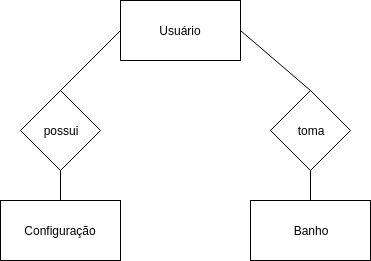
\includegraphics[width=0.6\linewidth]{figuras/ERPostgre.png}
	\caption{Modelo Entidade Relacionamento do PostgreSQL}
	\label{fig:erpostgre}
\end{figure}


\section{Configuração do InfluxDB}

Na configuração do InfluxDB, foi utilizada a biblioteca \textit{influx}\footnote{\url{https://www.npmjs.com/package/influx}}. Esta biblioteca permite a criação do banco de dados diretamente do código fonte do sistema, assim como as tabelas para guardar os dados temporais.

Foi criado o banco de dados \textit{water\_flow\_data}, que guarda os dados temporais dos banhos dos usuários. Neste banco, os dados são guardados com a \textit{tag} referente ao id do usuário cadastrado no banco relacional PostgreSQL. Os \textit{fields} são guardados os dados que chegam diretamente do sensor, que significa o fluxo de água naquele determinado instante.

O InfluxDB salva automaticamente os \textit{timestamps} de cada dado incluido nele, o que facilita a manipulação dos dados, pois não é necessário informar o \textit{timestamp} toda vez que for incluir algum dado no banco.

No \lstlistingname\ \ref{list:codigoinflux} está um exemplo do código de configuração e implementação das funções do InfluxDB no sistema.

%\begin{figure}[htbp]
%	\centering
%	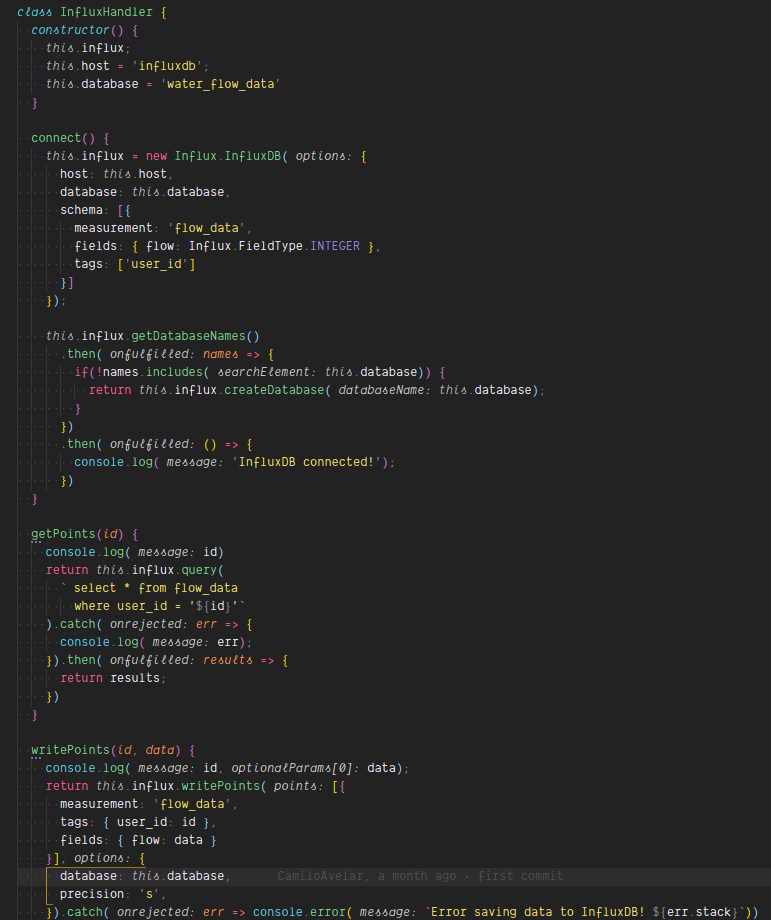
\includegraphics[width=1\linewidth]{figuras/influxconf.png}
%	\caption{Código de configuração do InfluxDB}
%	\label{fig:influxconf}
%\end{figure}

\begin{lstlisting}[label=list:codigoinflux, caption=Exemplo do código de configuração do InfluxDB]
const Influx = require('influx');

class InfluxHandler {
	constructor() {
		this.influx;
		this.host = 'influxdb';
		this.database = 'water_flow_data'
	}
	
	connect() {
		this.influx = new Influx.InfluxDB({
			host: this.host,
			database: this.database,
			schema: [{
				measurement: 'flow_data',
				fields: { flow: Influx.FieldType.INTEGER },
				tags: ['user_id']
			}]
		});
		
		this.influx.getDatabaseNames()
			.then(names => {
				if(!names.includes(this.database)) {
				return this.influx.createDatabase(this.database);
				}
			})
			.then(() => {
				console.log('InfluxDB connected!');
			})
	}
}
\end{lstlisting}

\section{Microsserviços}

Nesta seção são apresentadas as etapas de desenvolvimento dos microsserviços utilizados no sistema elaborado, assim como o serviço de simulação para viabilizar os testes e validação do sistema.

\subsection{\textit{Clean Architecture}}

Os microsserviços desenvolvidos foram projetados para seguir a \textit{Clean Architecture}. Esta arquitetura consiste em dividir as responsabilidades dentro de uma aplicação, encapsulando e abstraindo o código para facilitar a leitura e entendimento das devidas funções de cada arquivo.

É possível ver a divisão dos arquivos utilizando a \textit{Clean Architecture} do Sistema de Usuários na Figura \ref{fig:clean}. Explicando esta divisão, na pasta routes encontram-se as configuração das rotas que são utilizadas no sistema, nos \textit{controllers}, são feitas o tratamento dos \textit{inputs} e respostas das rotas, redirecionando para os interactors, que é onde está a lógica principal da aplicação. Nos \textit{repositories} é onde acontece a interação com o banco de dados, neste caso, com o PostgreSQL.

\begin{figure}[htbp]
	\centering
	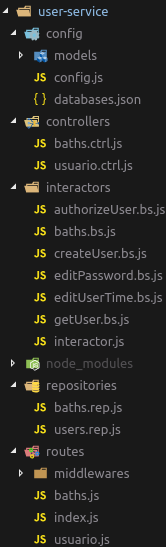
\includegraphics[width=0.25\linewidth]{figuras/cleanarch.png}
	\caption{Divisão dos arquivos do Sistema de Usuários}
	\label{fig:clean}
\end{figure}

\subsection{Sistema de usuários}

O propósito desta aplicação está em ter o controle e informações sobre o consumo de água em residências, para isso, é necessário ter um meio para conseguir as informações sobre os usuários do sistema. 

O microsserviço de usuários é responsável por cadastrar e editar usuários, cadastrar informações sobre o tempo de banho do usuário e autorizar o usuário a tomar o banho.

As operações são realizadas através dos \textit{endpoints}\footnote{Um \textit{endpoint} é uma forma de comunicação entre os sistemas, o sistema disponibiliza \textit{endpoints} que servem como como endereços para acesso ao sistema, que podem receber e enviar informações, dependendo do que foi programado.}, que são \textit{links} em que são passados parâmetros contendo a informação específica que o \textit{endpoint} requer.

Este microsserviço salva todos os dados recebidos nas tabelas do PostgreSQL.

O sistema possui os seguintes \textit{endpoints}:


\begin{itemize}
	\item /cadastrar: possibilita cadastrar o usuário com as informações do nome, senha e tempo de banho permitido.
	\item /autorizar: recebe o id do usuário e a senha, compara a senha enviada com a senha cadastrada e retorna se o usuário está ou não autorizado.
	\item /editar-tempo: possibilita editar o tempo de banho permitido do usuário.
	\item /editar-senha: possibilita editar a senha do usuário.
	\item /banho: salva no banco de dados informações do banho, o tempo e o usuário que tomou o banho.
	\item /banho/:id: retorna informações sobre todos os banhos do usuário.
\end{itemize}

Os códigos de implementação deste sistema podem ser observados no Apêndice A.

\subsection{Sistema de comunicação MQTT}

Este microsserviço é responsável pelo recebimento e manipulação dos dados recebidos dos sensores e do teclado numérico via MQTT. Também é responsável por comunicar com o sistema de usuários para a autorização do usuário, ligar ou desligar o atuador, além de salvar os dados no InfluxDB.

O sistema de comunicação recebe informações sobre as teclas digitadas e comunica com o sistema de usuários para autorizar ou não o ligamento do atuador, que significa o início do banho.

O sistema se subscreve nos seguintes tópicos do \textit{broker} MQTT para receber as informações:

\begin{itemize}
	\item \textit{keys}: é o tópico em que contém a tecla digitada no teclado numérico
	\item \textit{actuator}: é o tópico para enviar informações do atuador, para liga-lo ou desliga-lo
	\item \textit{user}: é o tópico para enviar informações do usuário, como o nome e se ele está autorizado ou não.
	\item \textit{sensor}: é o tópico para enviar informações do sensor de fluxo.
\end{itemize}

Os códigos de implementação deste sistema podem ser observados no Apêndice B.

\subsection{Sistema de simulação dos dados}

O sistema de simulação de dados emula todos os dados que podem ser capturados e enviados ao sistema físico, que são:

\begin{itemize}
	\item Dados do fluxo de água: informação recebida pelo sensor YF-S201;
	\item Dados do teclado numérico: informação de qual tecla foi pressionada no teclado;
	\item Informações para o atuador: informação para ligar/desligar o atuador;
\end{itemize}

Este sistema se inscreve nos tópicos do servidor MQTT e envia os dados simulados como se fosse o próprio sistema físico. Ao se iniciar o sistema, ele fica em estado de espera até alguma tecla for pressionada. Ao se pressionar uma tecla, ele a reconhece e toma as devidas ações, como requisitar a senha ou ligar/desligar o atuador.

Os dados do fluxo de água são número inteiros que são passados para o tópico do servidor MQTT, para simular estes dados envia-se um valor inteiro ao tópico em um intervalo pre-determinado de tempo (50 ms).

A Figura \ref{fig:mockservice} mostra o sistema de simulação funcionando, com o usuário com o id 3 sendo autorizado e o sinal de ligar/desligar o atuador enviado.

\begin{figure}[htbp]
	\centering
	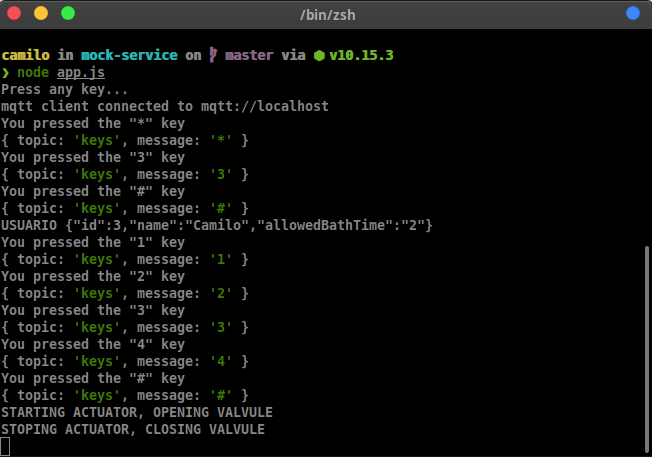
\includegraphics[width=0.6\linewidth]{figuras/mockservice.png}
	\caption{Exemplo do sistema de simulação}
	\label{fig:mockservice}
\end{figure}

\section{Configuração do HomeAssistant}

O HomeAssistant pode ser instalado a partir de diversos métodos\footnote{\url{https://www.home-assistant.io/docs/installation}}, neste sistema, a instalação foi feita utilizando o Hassbian, que é um sistema operacional linux para o RaspberryPi com o HomeAssistant pré-instalado.

Para configurar o HomeAssistant no RaspberryPi é necessário realizar o \textit{download} da imagem do Hassbian. Com o \textit{download} concluído, deve-se copiar a imagem para o cartão SD que será inserido no RaspberryPi. Para isto, utilizamos o \textit{balenaEtcher}.

Com a imagem devidamente escrita no cartão SD, basta inseri-lo no RaspberryPi, configurar a rede como descrito na Seção \ref{sec:confrasp}, e, ao iniciar o sistema, o HomeAssistant será carregado automaticamente.

O HomeAssistant utiliza a porta 8123 e, para conseguir visualizar sua interface, o IP deve ser acessado esta porta. No caso deste sistema, o IP do RaspberryPi foi colocado como estático \textit{192.168.2.60}, então, para acessar a interface deve-se estar conectado na mesma rede do RaspberryPi e acessar o link \textit{http://192.168.2.60:8123}, como podemos ver na Figura \ref{fig:homeassistanthome}.

\begin{figure}[htbp]
	\centering
	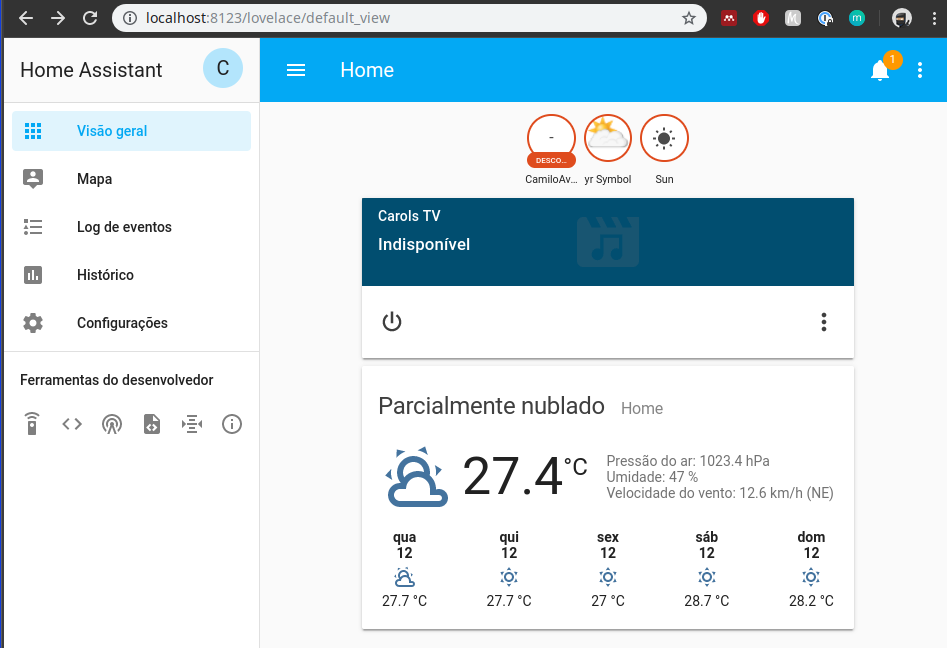
\includegraphics[width=1\linewidth]{figuras/homeassistanthome.png}
	\caption{Página inicial do HomeAssistant acessado por um cliente conectado na mesma rede local do servidor Hassbian}
	\label{fig:homeassistanthome}
\end{figure}

\subsection{Sensores}

A interface do HomeAssistant permite diversas configurações e inclusão de diferentes sensores, como mostra a Figura \ref{fig:homeassistant-dash}. No sistema desenvolvido neste trabalho, foi utilizado o sensor binário, que mostra o estado do chuveiro como ligado ou desligado. Cada usuário terá um sensor próprio, e seu estado será mostrado na interface.


\section{Configuração do Grafana}

A instalação do Grafana foi realizada através do \textit{download} e extração do pacote para o sistema operacional Debian.

Com o pacote devidamente instalado no sistema, o Grafana utiliza a porta 3003 como interface. Para acessar a sua interface, bastar acessar a porta 3003 do RaspberryPi, ou seja, acessar o link \textit{http://192.168.2.60:3003}, como na Figura \ref{fig:grafanahome}.

\begin{figure}[htbp]
	\centering
	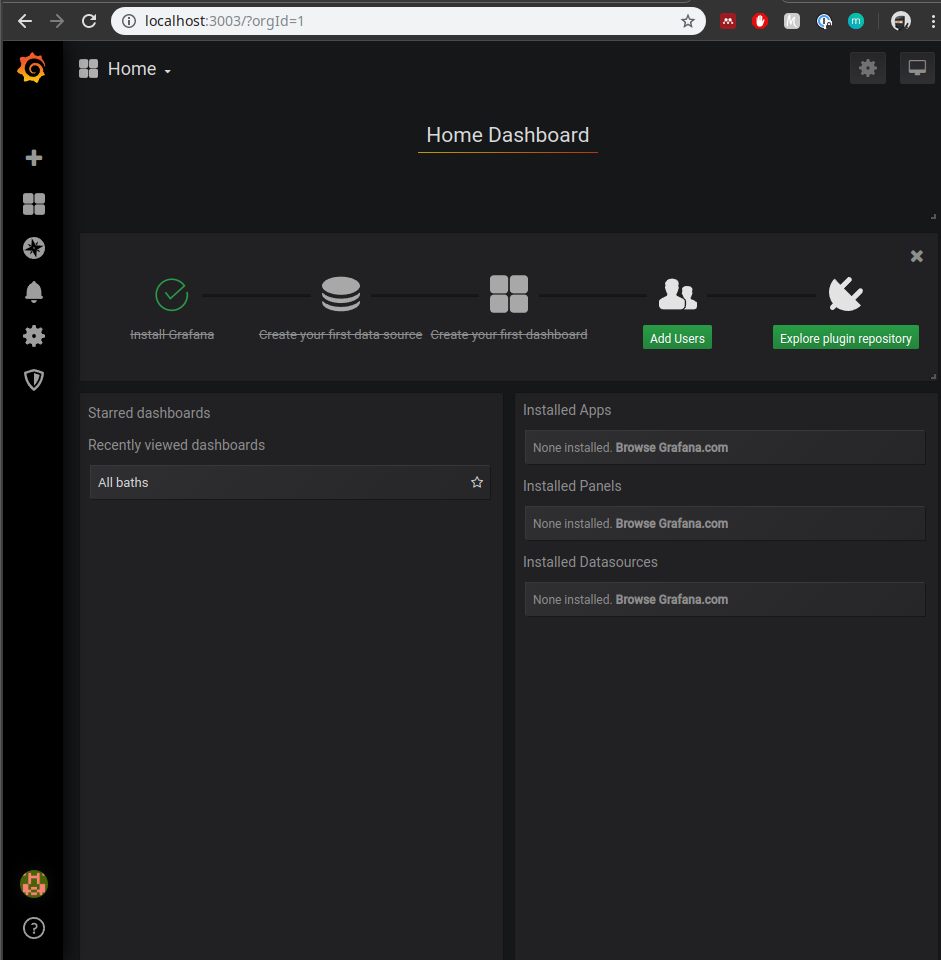
\includegraphics[width=1\linewidth]{figuras/grafanahome.png}
	\caption{Página inicial do Grafana}
	\label{fig:grafanahome}
\end{figure}

Ao acessar a interface do Grafana, é necessário criar um \textit{dashboard}\footnote{\textit{Dashboards} são painéis que mostram métricas e indicadores importantes para alcançar objetivos e metas traçadas de forma visual, facilitando a compreensão das informações geradas.} para a visualização dos dados do InfluxDB. Neste sistema criamos o \textit{dashboard AllBaths}, que se conecta no ip e porta do InfluxDB e realiza as consultas no banco \textit{water\_flow\_data} criado para guardar os dados temporais do fluxo de água.

A configuração do gráfico no Grafana pode ser observada na Figura \ref{fig:grafanaconf}.

\begin{figure}[htbp]
	\centering
	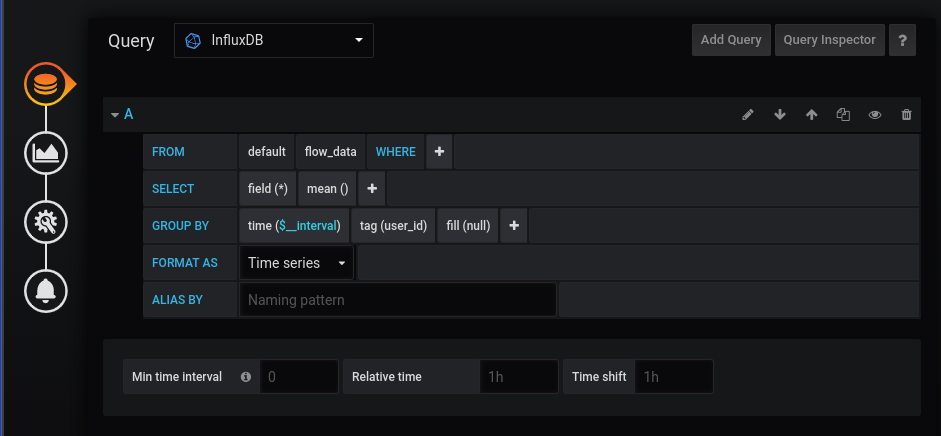
\includegraphics[width=1\linewidth]{figuras/grafanaconf.png}
	\caption{Configuração do gráfico no Grafana}
	\label{fig:grafanaconf}
\end{figure}

Após a configuração do \textit{dashboard}, um atalho será criado na página inicial do Grafana, e para visualizar os dados, basta clicar neste atalho e será aberto um gráfico com os fluxos medidos no sensor.

%\section{Configuração do Docker}
%
%Toda a configuração do Docker é realizada a partir do arquivo \textit{Dockerfile}, que deve ser criado no diretório do projeto em que se deseja configurar.
%
%No \textit{Dockerfile} alguns parâmetros devem ser passados para conseguir o resultado esperado, um deles é definir qual imagem do Docker será usada como base, no caso dos projetos desenvolvidos, todos utilizam o Node como imagem base, esta imagem é definida com o comando \textit{FROM node}.
%
%Outro parâmetro que precisa ser configurado é o \textit{WORKDIR}, que define o diretório que será usado como base dentro da imagem do Docker, no caso, dentro da imagem do Node.
%
%Um comando importante é o \textit{COPY}, que serve para copiar os arquivos do diretório raiz do Docker, para o \textit{WORKDIR} dentro da imagem do Node.
%
%Após copiar os arquivos, é necessário executar os comandos para instalar os pacotes dos projetos, com o comando \textit{RUN npm install}.
%
%Finalmente, deve-se definir um comando de entrada, que irá executar o projeto dentro da imagem no Docker, que é o comando \textit{CMD npm start}. Caso o projeto utilize alguma porta para configuração, deve-se também expor a porta para garantir o funcionamento com o comando \textit {EXPOSE numeroDaPorta}.
%
%O exemplo do \textit{Dockerfile} do Sistema de Usuários pode ser verificado na Figura \ref{fig:dockerfile}.
%
%\begin{figure}[htbp]
%	\centering
%	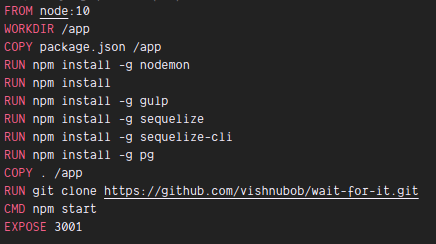
\includegraphics[width=0.7\linewidth]{figuras/dockerfile.png}
%	\caption{Exemplo de \textit{Dockerfile} do Sistema de Usuários}
%	\label{fig:dockerfile}
%\end{figure}
%
%\subsection{Docker-compose}
%
%O \textit{Dockerfile} permite a execução única do projeto em que ele está presente, para iniciar os projetos utilizando apenas o \textit{Dockerfile} é necessário iniciar um por um.
%
%Para contornar este problema, o \textit{docker-compose} permite a execução de todos os projetos com apenas um comando, desde que um arquivo \textit{docker-compose.yml} esteja devidamente configurado. Este arquivo permite também a instalação e configuração automática de todos os programas utilizados neste trabalho, como o PostgreSQL, o InfluxDB, o Grafana e o Mosquitto.
%
%A configuração do \textit{docker-compose.yml} é simples como a do \textit{Dockerfile}, nele, deve-se especificar a versão que deseja utilizar, neste projeto foi utilizada a 3.5, com o comando \textit{version}:"3.5".
%
%Após a definição da versão, deve-se especificar os \textit{services}, que são as imagens que devem iniciar com o Docker. Neste projeto foram utilizados os \textit{builds} dos projetos já implementados com os devidos \textit{Dockerfiles} configurados. 
%
%Além dos projetos já implementados, foram especificados também os programas que foram utilizados no sistema, com o comando \textit{image:}postgres, \textit{image:}homeassistant, \textit{image:}eclipse-mosquitto, \textit{image:}grafana, \textit{image:}influxdb.
%
%O código implementado do \textit{docker-compose.yml} do projeto pode ser verificado no Apêndice C.



